\subsubsection{Ruční návrh}
Pro vstupní větev je stanoven proud \qty{50}{\micro\ampere}, výpočet rozměrů je proveden obdovným způsobem jako v minulém přkladu:
\[
    \frac{W_{3,5}}{L_{3,5}}=\frac{2\cdot I_{D3}}{KP_{P}\cdot (U_{GS} -U_{TH})^2 } 
\]
\[
    \frac{W_{3,5}}{L_{3,5}}=\frac{2\cdot \num{50e-6}}{\num{60e-6} \cdot (\num{0.2})^2 } 
\]
\[
    \frac{W_{3,5}}{L_{3,5}}=\num{41,67}
\]

Opět použijeme délku kanálu \(L_{3,5}=L_{4,6} = \qty{2}{\micro\meter}\), tedy \(W_{3,5} =\qty[round-mode=places,round-precision=2]{83,34}{\micro\meter}\). Druhý tranzistor má dosáhnout dvakrát vyššího proudu, takže zvolíme \(W_{4,6} =\qty{166,68}{\micro\meter}\)  

Pro nastavení proudu slouží rezistor R2. Jeho hodnota je stanovena na základě úbytku napětí na rezistoru.
% U_bs pro M3 je U_GS1 coz je U_th0 + U_ov
% z tabulky pak odecitam radek pro nejvyssi U_bs, coz je porad mene...
% zaokrouhleno nahoru 600m
\begin{align*}
    U_{R 2}=&U_{C C}-U_{G S 3}-U_{G S 5} \\
           =&U_{C C}-U_{T H 0,3}- U_{O V 3}-U_{T H, 5}-U_{O V 5} \\
           =&U_{C C}-U_{T H 0,3}-U_{T H, 5}-2 \cdot U_{O V 3,5} \\
           =&\num{1.8}-\num{0.4433}-\num{0.6}-2 \cdot \num{0.2} \\
           =&\qty{0.3567}{\volt}
\end{align*}

\begin{align*}
    R_{2} =& \frac{U_{R1}}{I_{M1} } \\
          =& \frac{\num{0.3567}}{\num{50e-6}} \\
          =& \qty{7.134}{\kilo\ohm}
\end{align*}

Pro výpočet výstupního odporu použijeme zjednodušený vztah, jelikož rozměry tranzistorů \(M4\) a \(M6\) jsou stejné:
\begin{align*}
    r_{OUT} =& r_{o4,6}^2 \cdot g_{m6} \\
            =& \left(\frac{1}{\lambda_{PMOS} \cdot I_{M6} }\right)^2 \cdot \frac{2\cdot I_{M6}}{U_{OV6} } \\
            =& \frac{2}{\lambda_{PMOS}^2 \cdot I_{M6} \cdot U_{OV6} } \\
            =& \frac{2}{\num{0.079}^2 \cdot \num{100e-6} \cdot \num{0.2}} \\
            =& \qty{16.02}{\mega\ohm}
\end{align*}

\subsubsection{Výstupní charakteristika}
\begin{figure}[h!]
    \centering
    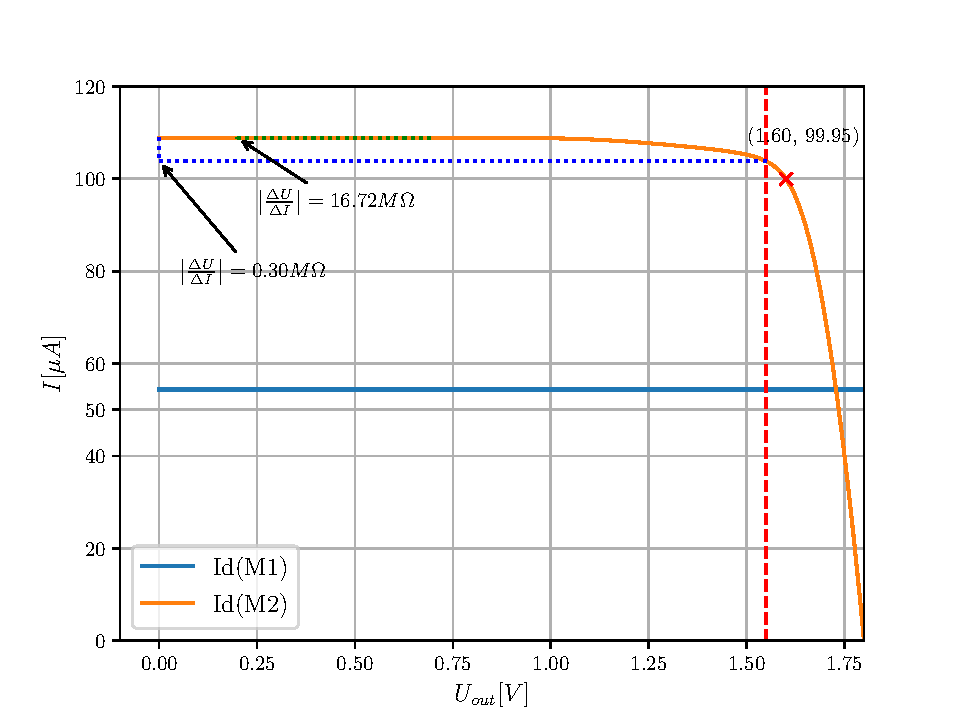
\includegraphics[width=0.8\textwidth]{2-2.pdf}
    \caption{DC analýza pro kaskodové proudové zrcadlo.}
    \label{fig:2-2-pdf}
\end{figure}